Po podstawowe definicje, czym są termy lambda, odsyłam do notatek z ćwiczeń.

Podstawienie \( M[x := n] \) oznacza term powstały z \( M \) poprzez zastąpienie wszystkich wolnych wystąpień \( x \) przez \( N \).

\subsubsection*{\( \alpha \)-konwersja}
Operacja zmiany nazw zmiennych związanych
\begin{align*}
    & M =_{\alpha} M \\
    & \lambda x.M =_{\alpha} \lambda y.M[x := y] \quad \text{dla } y \notin FV(M)
\end{align*}

\subsubsection*{\( \beta \)-redukcja}
Operacja przekształcenia termu w postaci \textbf{redeks} (\((\lambda x.M)N\)) poprzez zastąpienie wolnych wystąpień zmiennej argumentem
\[ (\lambda x.M)N \rightarrow_{\beta} M[x := N] \]
Warunek: żadna zmienna z \( FV(N) \) nie zostanie związana po podstawieniu do \( M \).

Przykład, jak nie można:
\[ (\lambda xy.xy)y \xrightarrow[]{{\color{red} \times}}_{\beta} \lambda y.yy \]
Należy wcześniej zastosować \( \alpha \)-konwersję.
\[ (\lambda xy.xy)y =_{\alpha} (\lambda xz.xz)y \rightarrow_{\beta} \lambda z.yz \]

Jeśli \( M \rightarrow_{\beta} N \), to
\begin{itemize}
    \item \( \lambda x.M \rightarrow_{\beta} \lambda x.N \)
    \item \( MK \rightarrow_{\beta} NK \)
    \item \( KM \rightarrow_{\beta} KN \)
\end{itemize}

Definiujemy: \\
\( \twoheadrightarrow_{\beta} \) domknięcie przechodnie i zwrotne relacji \( \rightarrow_{\beta} \cup =_{\alpha} \), \\
\( =_{\beta} \) domknięcie symetryczne relacji \( \twoheadrightarrow_{\beta} \).

\begin{theorem}[Church-Rosser, 1936]
    Dla dowolnych termów \( M, \ N, \ K \), które spełniają \( M \twoheadrightarrow_{\beta} N \) i \( M \twoheadrightarrow_{\beta} K \) istnieje term \( L \) taki, że \( N \twoheadrightarrow_{\beta} L \) i \( K \twoheadrightarrow_{\beta} L \).
    \begin{center}
        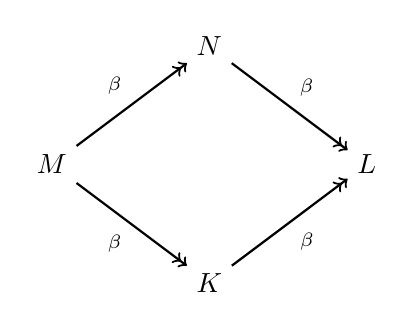
\begin{tikzpicture}[
    node distance=3cm,
    surj/.style={->>, line width=0.8pt}
    ]
    
    \node (M) at (0,0) {\(M\)};
    \node (N) at (2,1.5) {\(N\)};
    \node (K) at (2,-1.5) {\(K\)};
    \node (L) at (4,0) {\(L\)};
        
    \draw[surj] (M) -- node[above left]{\(\scriptstyle \beta\)} (N);
    \draw[surj] (M) -- node[below left]{\(\scriptstyle \beta\)} (K);
    \draw[surj] (N) -- node[above right]{\(\scriptstyle \beta\)} (L);
    \draw[surj] (K) -- node[below right]{\(\scriptstyle \beta\)} (L);
    
\end{tikzpicture}
    \end{center}
\end{theorem}

\begin{theorem}[O zygzaku, Church-Rosser]
    Jeśli \( M =_{\beta} N \), to istnieje zygzak.
\end{theorem}
\begin{proof}[Szkic]
    Wynika z poprzedniego twierdzenia.
    \begin{center}
        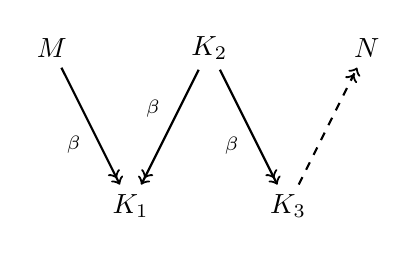
\begin{tikzpicture}[
    surj/.style={->>, line width=0.8pt},
    dashedsurj/.style={->>, dashed, line width=0.8pt}
    ]

    \node (M) at (0,2) {\(M\)};
    \node (K1) at (1,0) {\(K_1\)};
    \node (K2) at (2,2) {\(K_2\)};
    \node (K3) at (3,0) {\(K_3\)};
    \node (N) at (4,2) {\(N\)};
    
    \draw[surj] (M) -- node[below left]{\(\scriptstyle \beta\)} (K1);
    \draw[surj] (K2) -- node[above left]{\(\scriptstyle \beta\)} (K1);
    \draw[surj] (K2) -- node[below left]{\(\scriptstyle \beta\)} (K3);
    \draw[dashedsurj] (K3) -- (N);

\end{tikzpicture}
    \end{center}
\end{proof}

\begin{theorem}[Church-Rosser]
    Dla dowolnych termów \( M =_{\beta} N \) istnieje \( L \), dla którego \( M \twoheadrightarrow_{\beta} L \twoheadleftarrow_{\beta} N \).
\end{theorem}
\begin{proof}[Szkic]
    Wynika z poprzedniego twierdzenia.
    \begin{center}
        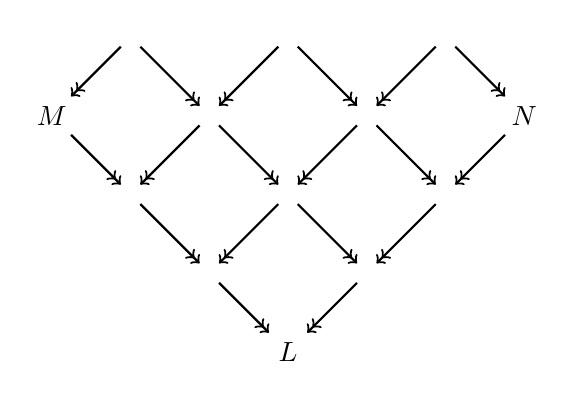
\begin{tikzpicture}[
    surj/.style={->>, line width=0.8pt},
    dashedsurj/.style={->>, dashed, line width=0.8pt}
    ]

    \node (K1) at (1,4) {};
    \node (K2) at (3,4) {};
    \node (K3) at (5,4) {};
    \node (M) at (0,3) {\(M\)};
    \node (K4) at (2,3) {};
    \node (K5) at (4,3) {};
    \node (N) at (6,3) {\(N\)};
    \node (K6) at (1,2) {};
    \node (K7) at (3,2) {};
    \node (K8) at (5,2) {};
    \node (K9) at (2,1) {};
    \node (K10) at (4,1) {};
    \node (L) at (3,0) {\(L\)};
    
    \draw[surj] (K1) -- (M);   \draw[surj] (K1) -- (K4);
    \draw[surj] (K2) -- (K4);  \draw[surj] (K2) -- (K5);
    \draw[surj] (K3) -- (K5);  \draw[surj] (K3) -- (N);
    \draw[surj] (M) -- (K6);
    \draw[surj] (N) -- (K8);
    \draw[surj] (K4) -- (K7);  \draw[surj] (K4) -- (K6);
    \draw[surj] (K5) -- (K7);  \draw[surj] (K5) -- (K8);
    \draw[surj] (K6) -- (K9);
    \draw[surj] (K7) -- (K9);  \draw[surj] (K7) -- (K10);
    \draw[surj] (K8) -- (K10);
    \draw[surj] (K9) -- (L);
    \draw[surj] (K10) -- (L);

\end{tikzpicture}
    \end{center}
\end{proof}

Term \( M \) jest w formie normalnej, jeśli nie posiada redeksów.

\begin{theorem}[O formie normalnej, Church-Rosser]
    Dla dowolnych termów \( M, \ N, \ K \), które spełniają \( M \twoheadrightarrow_{\beta} N \) i \( M \twoheadrightarrow_{\beta} K \), jeśli \( N \) i \( K \) są normalne, to \( N =_{\beta} K \).
\end{theorem}
\begin{proof}[Szkic]
    Na mocy pierwszego twierdzenia Churcha-Rossera istnieje \( L \) takie, że \( N \twoheadrightarrow_{\beta} L \) i \( K \twoheadrightarrow_{\beta} L \).
    Skoro \( N \) i \( K \) są normalne, to nie zawierają redeksów, więc dalsze \( \beta \)-redukcje są niemożliwe, czyli \( N \twoheadrightarrow_{\alpha} L \) i \( K \twoheadrightarrow_{\alpha} L \), a zatem \( N =_{\beta} K \).
    \begin{center}
        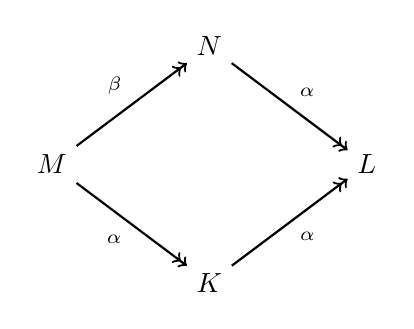
\begin{tikzpicture}[
    node distance=3cm,
    surj/.style={->>, line width=0.8pt}
    ]
    
    \node (M) at (0,0) {\(M\)};
    \node (N) at (2,1.5) {\(N\)};
    \node (K) at (2,-1.5) {\(K\)};
    \node (L) at (4,0) {\(L\)};
        
    \draw[surj] (M) -- node[above left]{\(\scriptstyle \beta\)} (N);
    \draw[surj] (M) -- node[below left]{\(\scriptstyle \alpha\)} (K);
    \draw[surj] (N) -- node[above right]{\(\scriptstyle \alpha\)} (L);
    \draw[surj] (K) -- node[below right]{\(\scriptstyle \alpha\)} (L);
    
\end{tikzpicture}
    \end{center}
\end{proof}
\subsection*{Ważne termy}
\begin{itemize}
    \item \(K = \lambda xy.x = \pi_i\) 
    \item \(K^* = \lambda xy.y = \pi_2\)
    \item Para uporządkowana:
    \[ \lambda yzx.xyz=U \] 
    \[ [p,q] = Upq = \lambda x.x pq \]
    \[ [p,q]\pi_1 = p \qquad [p,q]\pi_2=q \]
    \item \(S = \lambda xyz,xz(yz)\)
    \item \(\omega = \lambda x.xx\)
    \item \(\Omega = \omega \omega = (\lambda y.yy)(\lambda x.xx) \to_{\beta} (\lambda x.xx)(\lambda x.xx) \to_{\beta} \dots \) najprostszy term bez postaci normalnej
    \item Operator punktu stałego \(Y\) to taki term, że dla każdego termu \(M\)
    \[ YM =_\beta M(YM) \]
    najkrótszym operatorem punktu stałego (potwierdzone bruteforcem) jest:
    \[ Y = \lambda y(\lambda x.y(xx))(\lambda x.y(xx)) \]
\end{itemize}

\section{Numerale Churcha}
Numerale Churcha reprezentują liczby naturalne w rachunku lambda, można by je zdefiniować inaczej, ale tak jest wygodnie.
\\

Definiujemy liczby naturalne jako
\[ 0\equiv\lambda sz.z \]
\[ 1 \equiv \lambda sz.sz \]
\[ n \equiv \lambda sz. \underbrace{s(s\dots(s}_{\text{n razy s}}z)) \]
Interpretacja jest taka, że bierzemy termy \(z\) reprezentujący zero oraz \(s\) reprezentujący następnik i aplikujemy następnik \(n\) razy do zera. \\
Numerale Churcha są w postaci normalnej więc \(i \neq j \Rightarrow i \neq_\beta j\).
